\documentclass[final]{beamer}
\usetheme{RJH}
\usepackage[orientation=portrait,size=a1,scale=1.3,debug]{beamerposter}
\usepackage[absolute,overlay]{textpos}
\usepackage{amsmath}
\usepackage{mathtools}
\usepackage{commath}
\usepackage[font=scriptsize,labelfont=bf]{caption}
\setlength{\TPHorizModule}{1cm}
\setlength{\TPVertModule}{1cm}
\setbeamertemplate{caption}[numbered]
\setbeamertemplate{itemize items}[ball]

\title{Dynamical systems modeling of the child–mother dyad:\\ \vspace{0.15em}
Causality between child-directed language complexity \\ 
\vspace{0.15em}
and language development \vspace{0.15em}}
%\author{{\large \bf Jeremy Irvin \qquad Daniel Spokoyny} \\
%\vspace{0.2em}
%  College of Creative Studies\\ \vspace{0.2em}
%  {\large \bf Ferm\'{\i}n Moscoso del Prado Mart\'{\i}n } \\ \vspace{0.3em}
%  Department of Linguistics}
\footer{}
\author[shortname]{Jeremy Irvin 
%\inst{1} 
\and Daniel Spokoyny 
%\inst{1} 
\and Ferm\'{\i}n Moscoso del Prado Mart\'{\i}n 
%\inst{2}
}
%\institute[shortinst]{\inst{1} College of Creative Studies \and %
%                      \inst{2} Department of Linguistics}
\date{}

\begin{document}
\begin{frame}{} 

\begin{textblock}{10}(1,4.5)

\includegraphics[width=6.5cm]{ccs.png}
\end{textblock}

\begin{textblock}{10}(50,4.8)

\includegraphics[width=8.5cm]{ling.jpg}
\end{textblock}

\begin{textblock}{28}(1,9)
\begin{block}{Abstract}
We model the \emph{causal} links between child language (CL) and child-directed language (CDL). We take pairs of sequences of linguistic measurements from a longitudinal study. Each child- mother pair of sequences is considered as an instance of the trajectory of a high-dimensional dynamical system. We then use Multispatial Convergent Cross Mapping to ascertain the directions of causality between the pairs of sequences, that is, whether the complexity of CL drives that of CDL, the complexity of CDL drives that of CL, both, or neither.
\end{block}

\begin{block}{Background}

\begin{itemize}
\item \text{ }Child-directed language (``motherese'')
\item \text{ }Fine-tuning 
\begin{itemize}
\item \text{ }Weak or Strong
\end{itemize}
\end{itemize}
\hrule
\begin{itemize}
\item \text{ }Dynamical systems models describe the co-evolution of multiple variables over time

\item \text{ }Typically described by a system of coupled differential equations
\item \text{ }Linguistic and behavioral interaction between parent-child dyads can be jointly considered as part of a single dynamical system
\end{itemize}
\begin{figure}
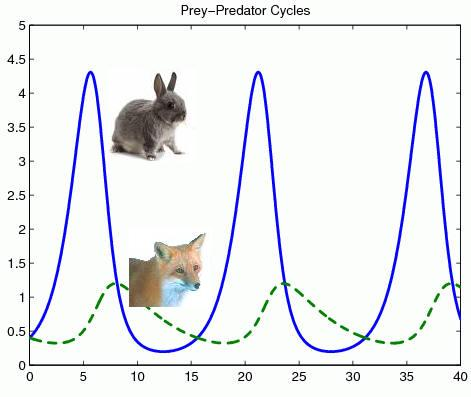
\includegraphics[width=10cm]{pred_prey.jpg}
\caption{Poop}
\label{fig:predprey}
\end{figure}
\end{block}

\begin{block}{Causality Detection in Dynamical Systems}
\begin{figure}
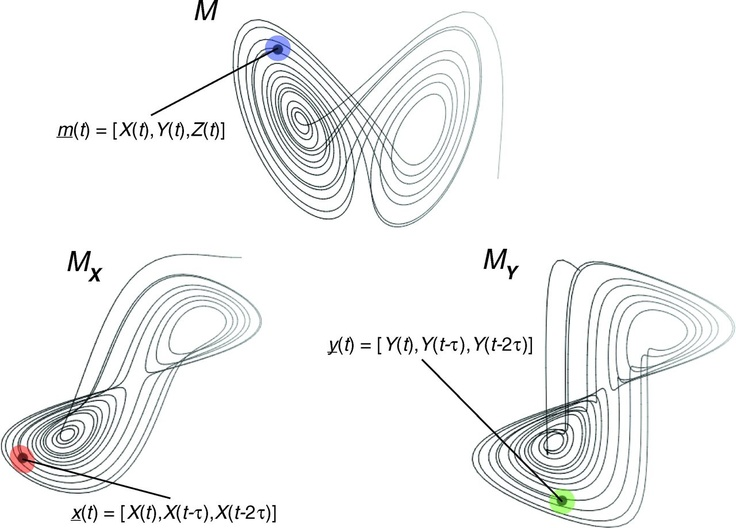
\includegraphics[width=15cm]{lorenz2.jpg}
\caption{Reconstructed manifold for Lorenz’s system ($M$; top), as well as the shadow manifolds reconstructed considering only $X$ ($M_X$ ; bottom-left) and $Y$ ($M_Y$ ; bottom-right) (Sugihara et al., 2012).}
\label{fig:lorenz}
\end{figure}

\small
\begin{equation}
\begin{dcases}
\dod{X}{t} = \sigma ( Y - X ) \\[10pt]
\dod{Y}{t} = X (\rho - Z) - Y \\[10pt]
\dod{Z}{t} = X Y - \beta Z 
\end{dcases}.
\label{eq:lorenz}
\end{equation}
\normalsize 
\end{block}
\end{textblock}

\begin{textblock}{28}(30.5,9)
\begin{block}{Methods and Materials}
\begin{figure}
\begin{tabular}{ccc}
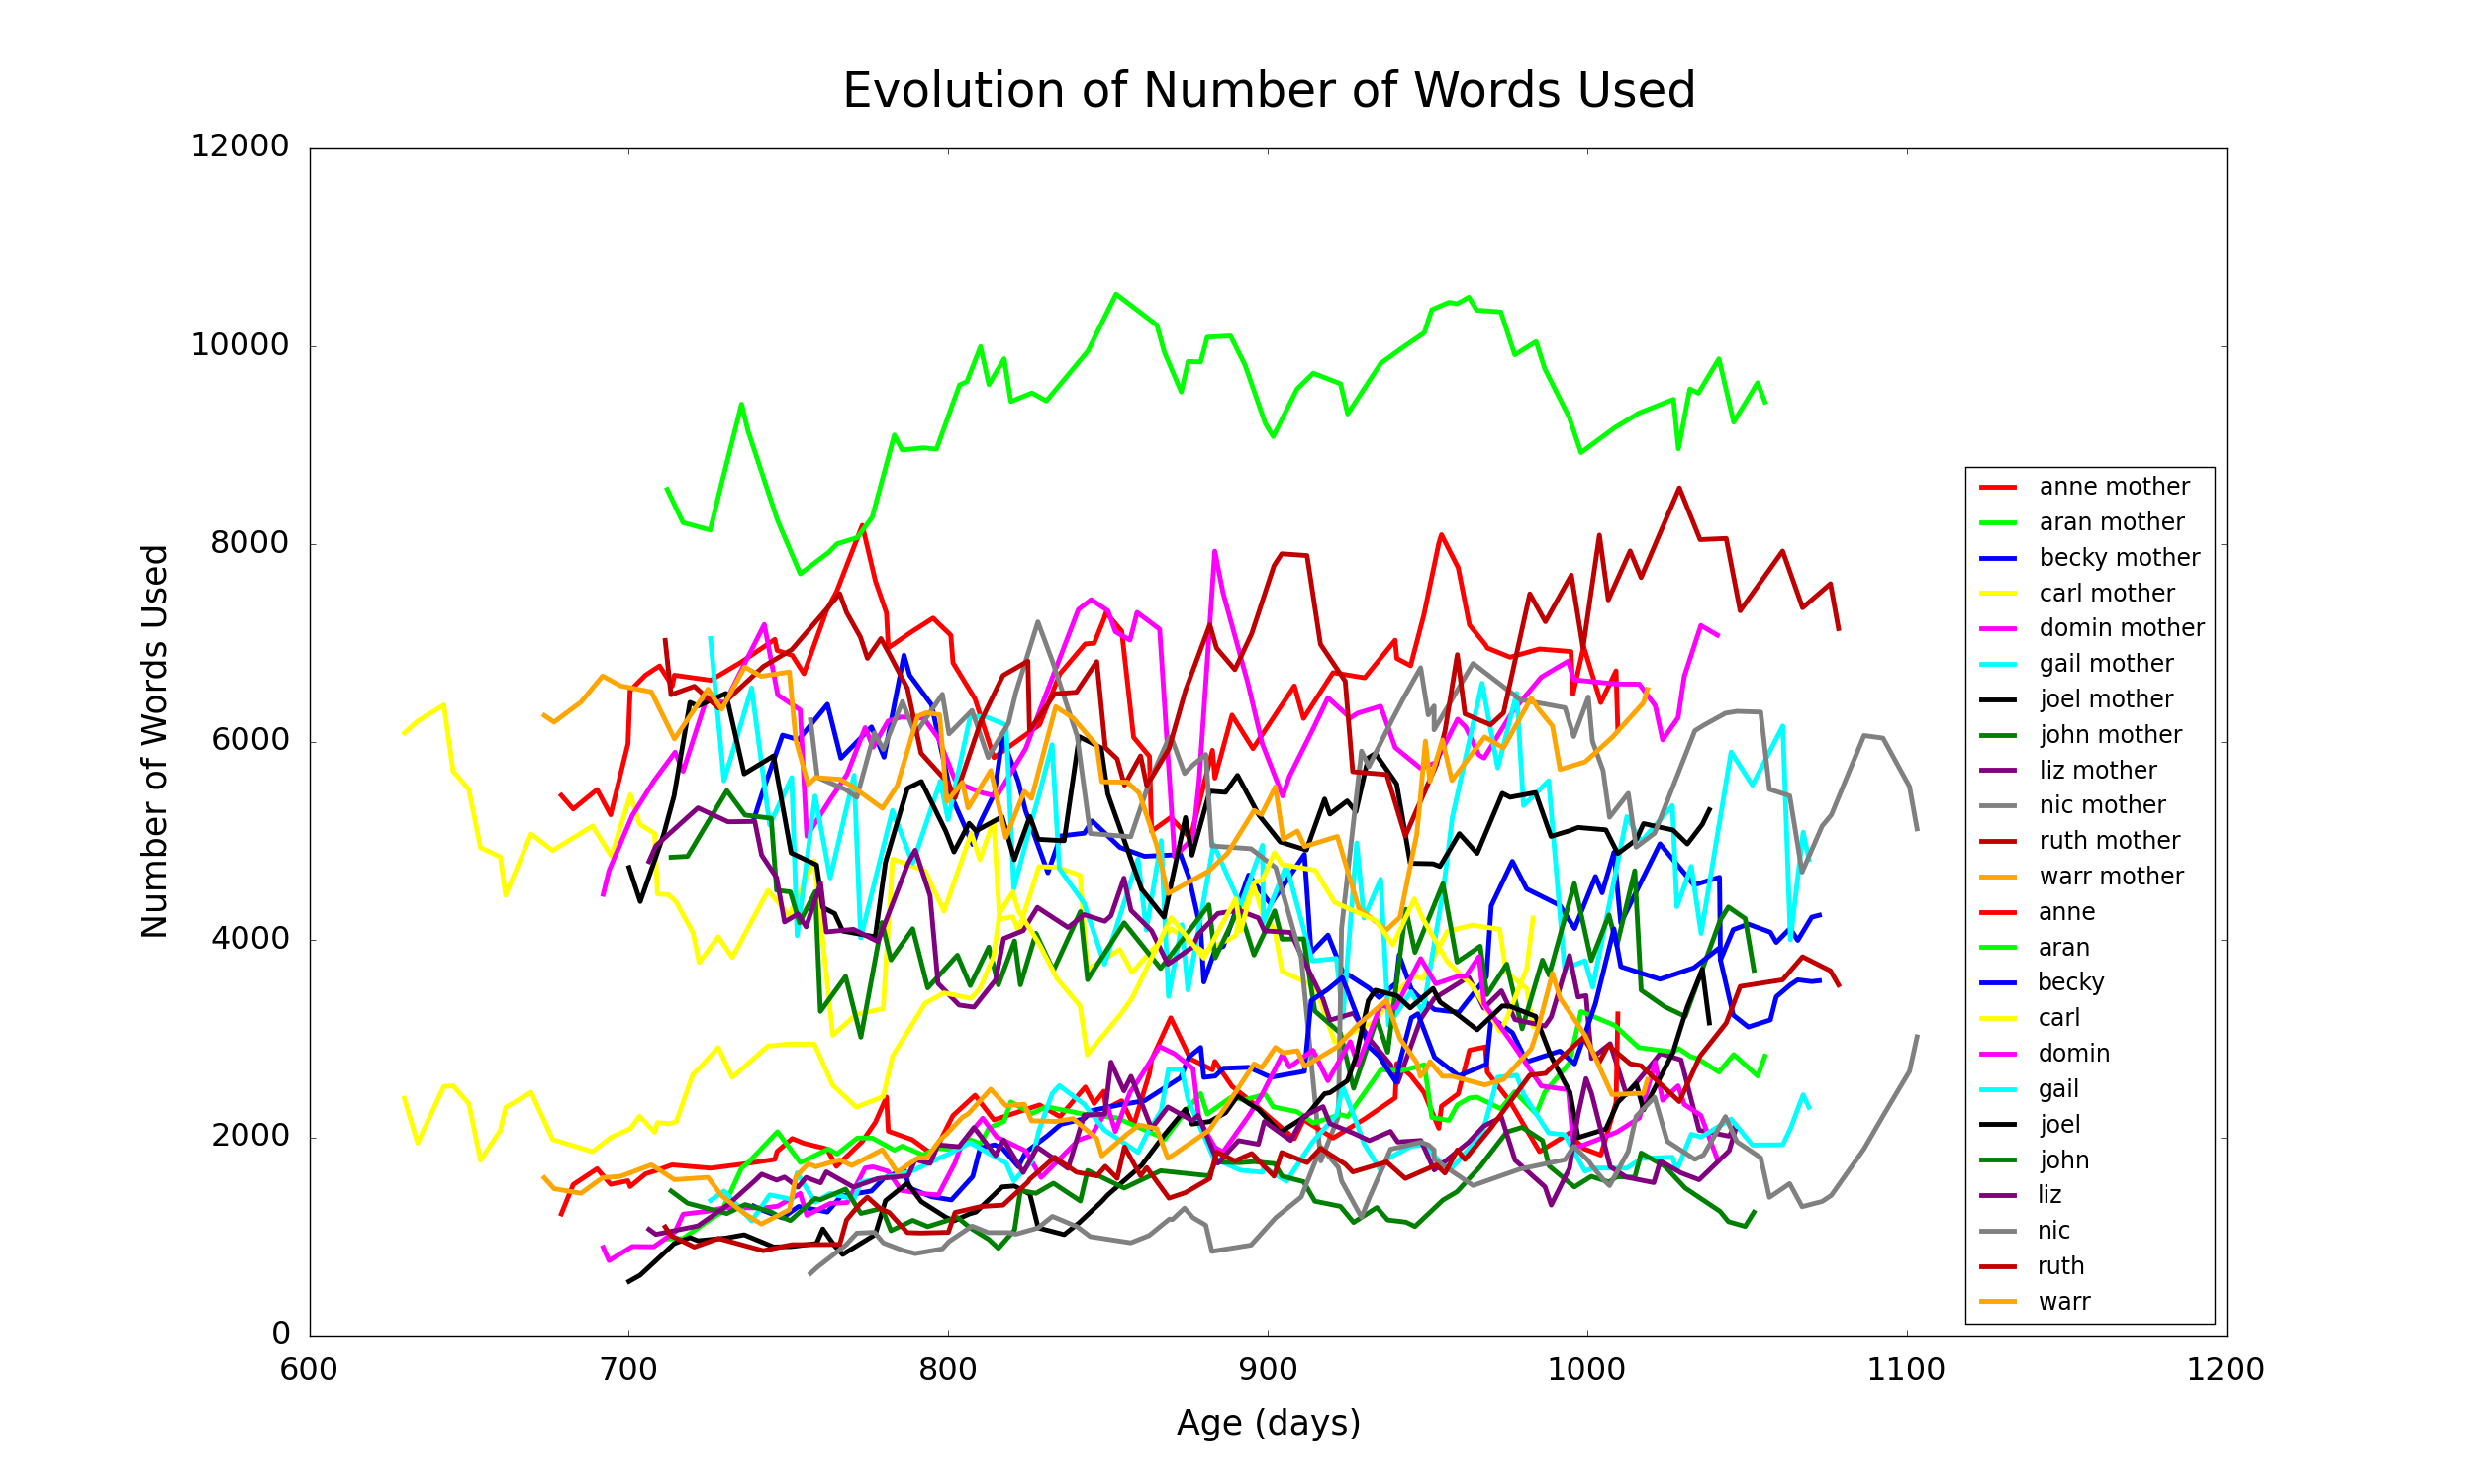
\includegraphics[width=.325\textwidth]{nwords_evolution.png} &
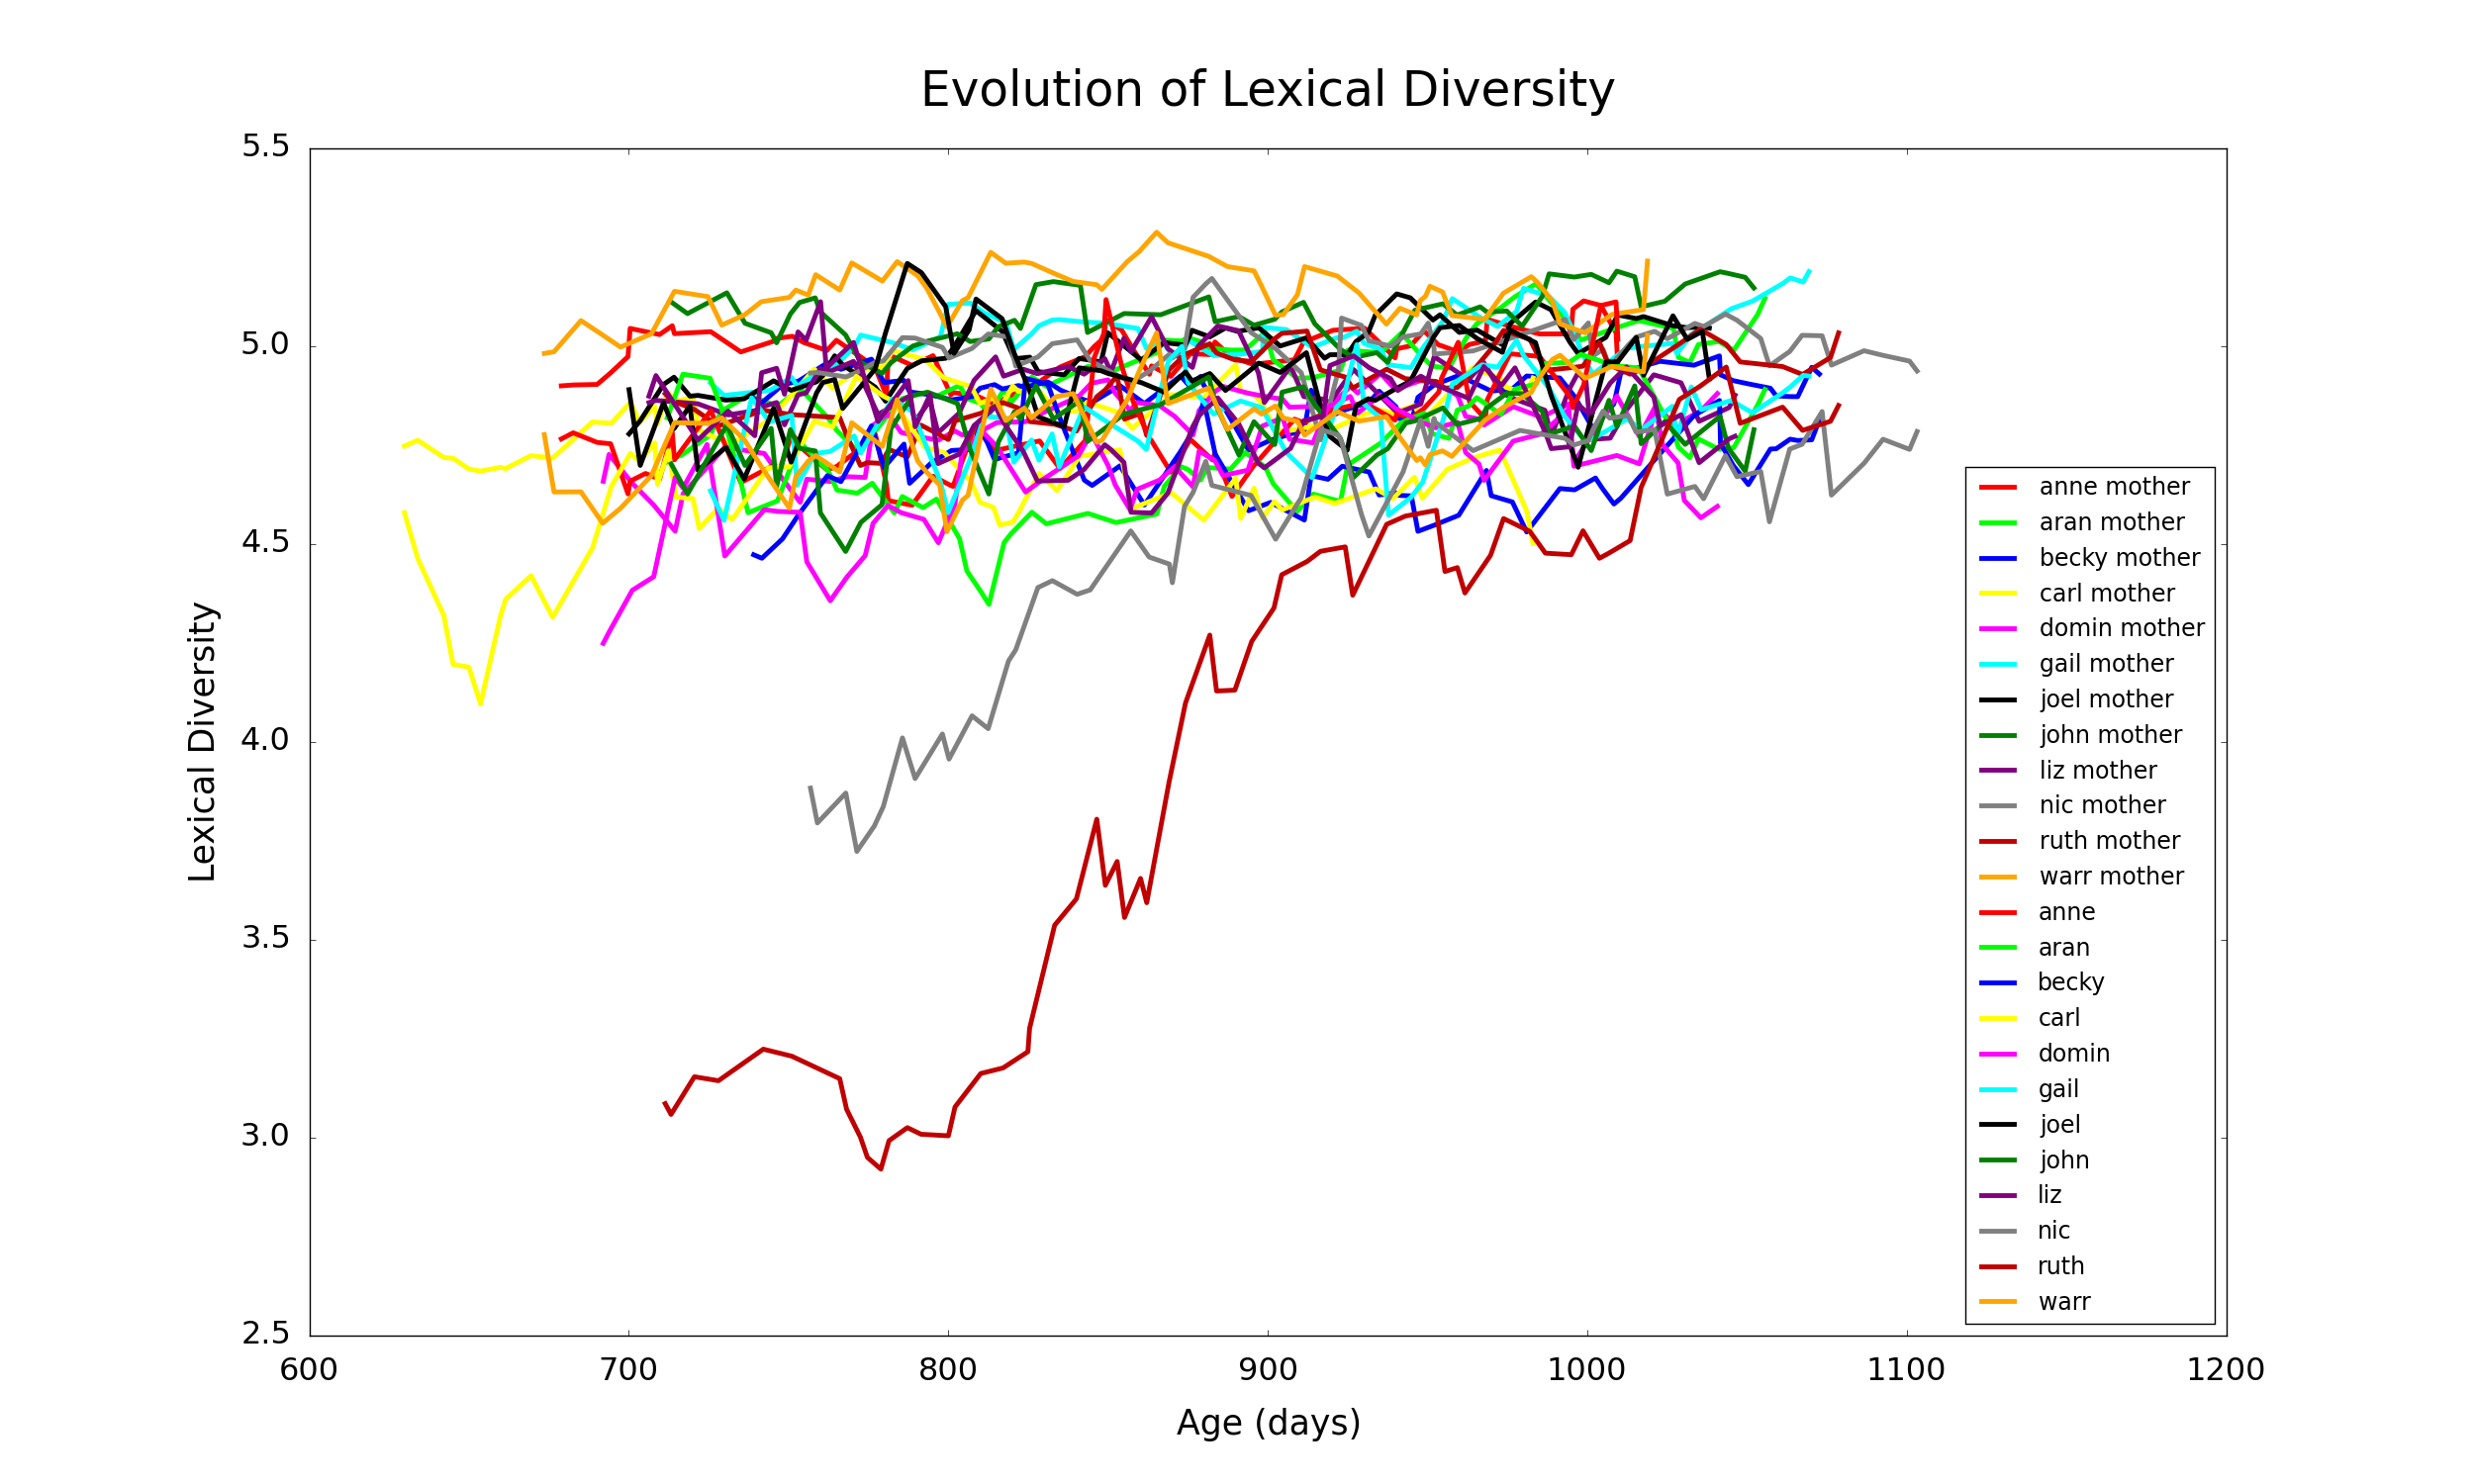
\includegraphics[width=.325\textwidth]{lexical_evolution.png} &
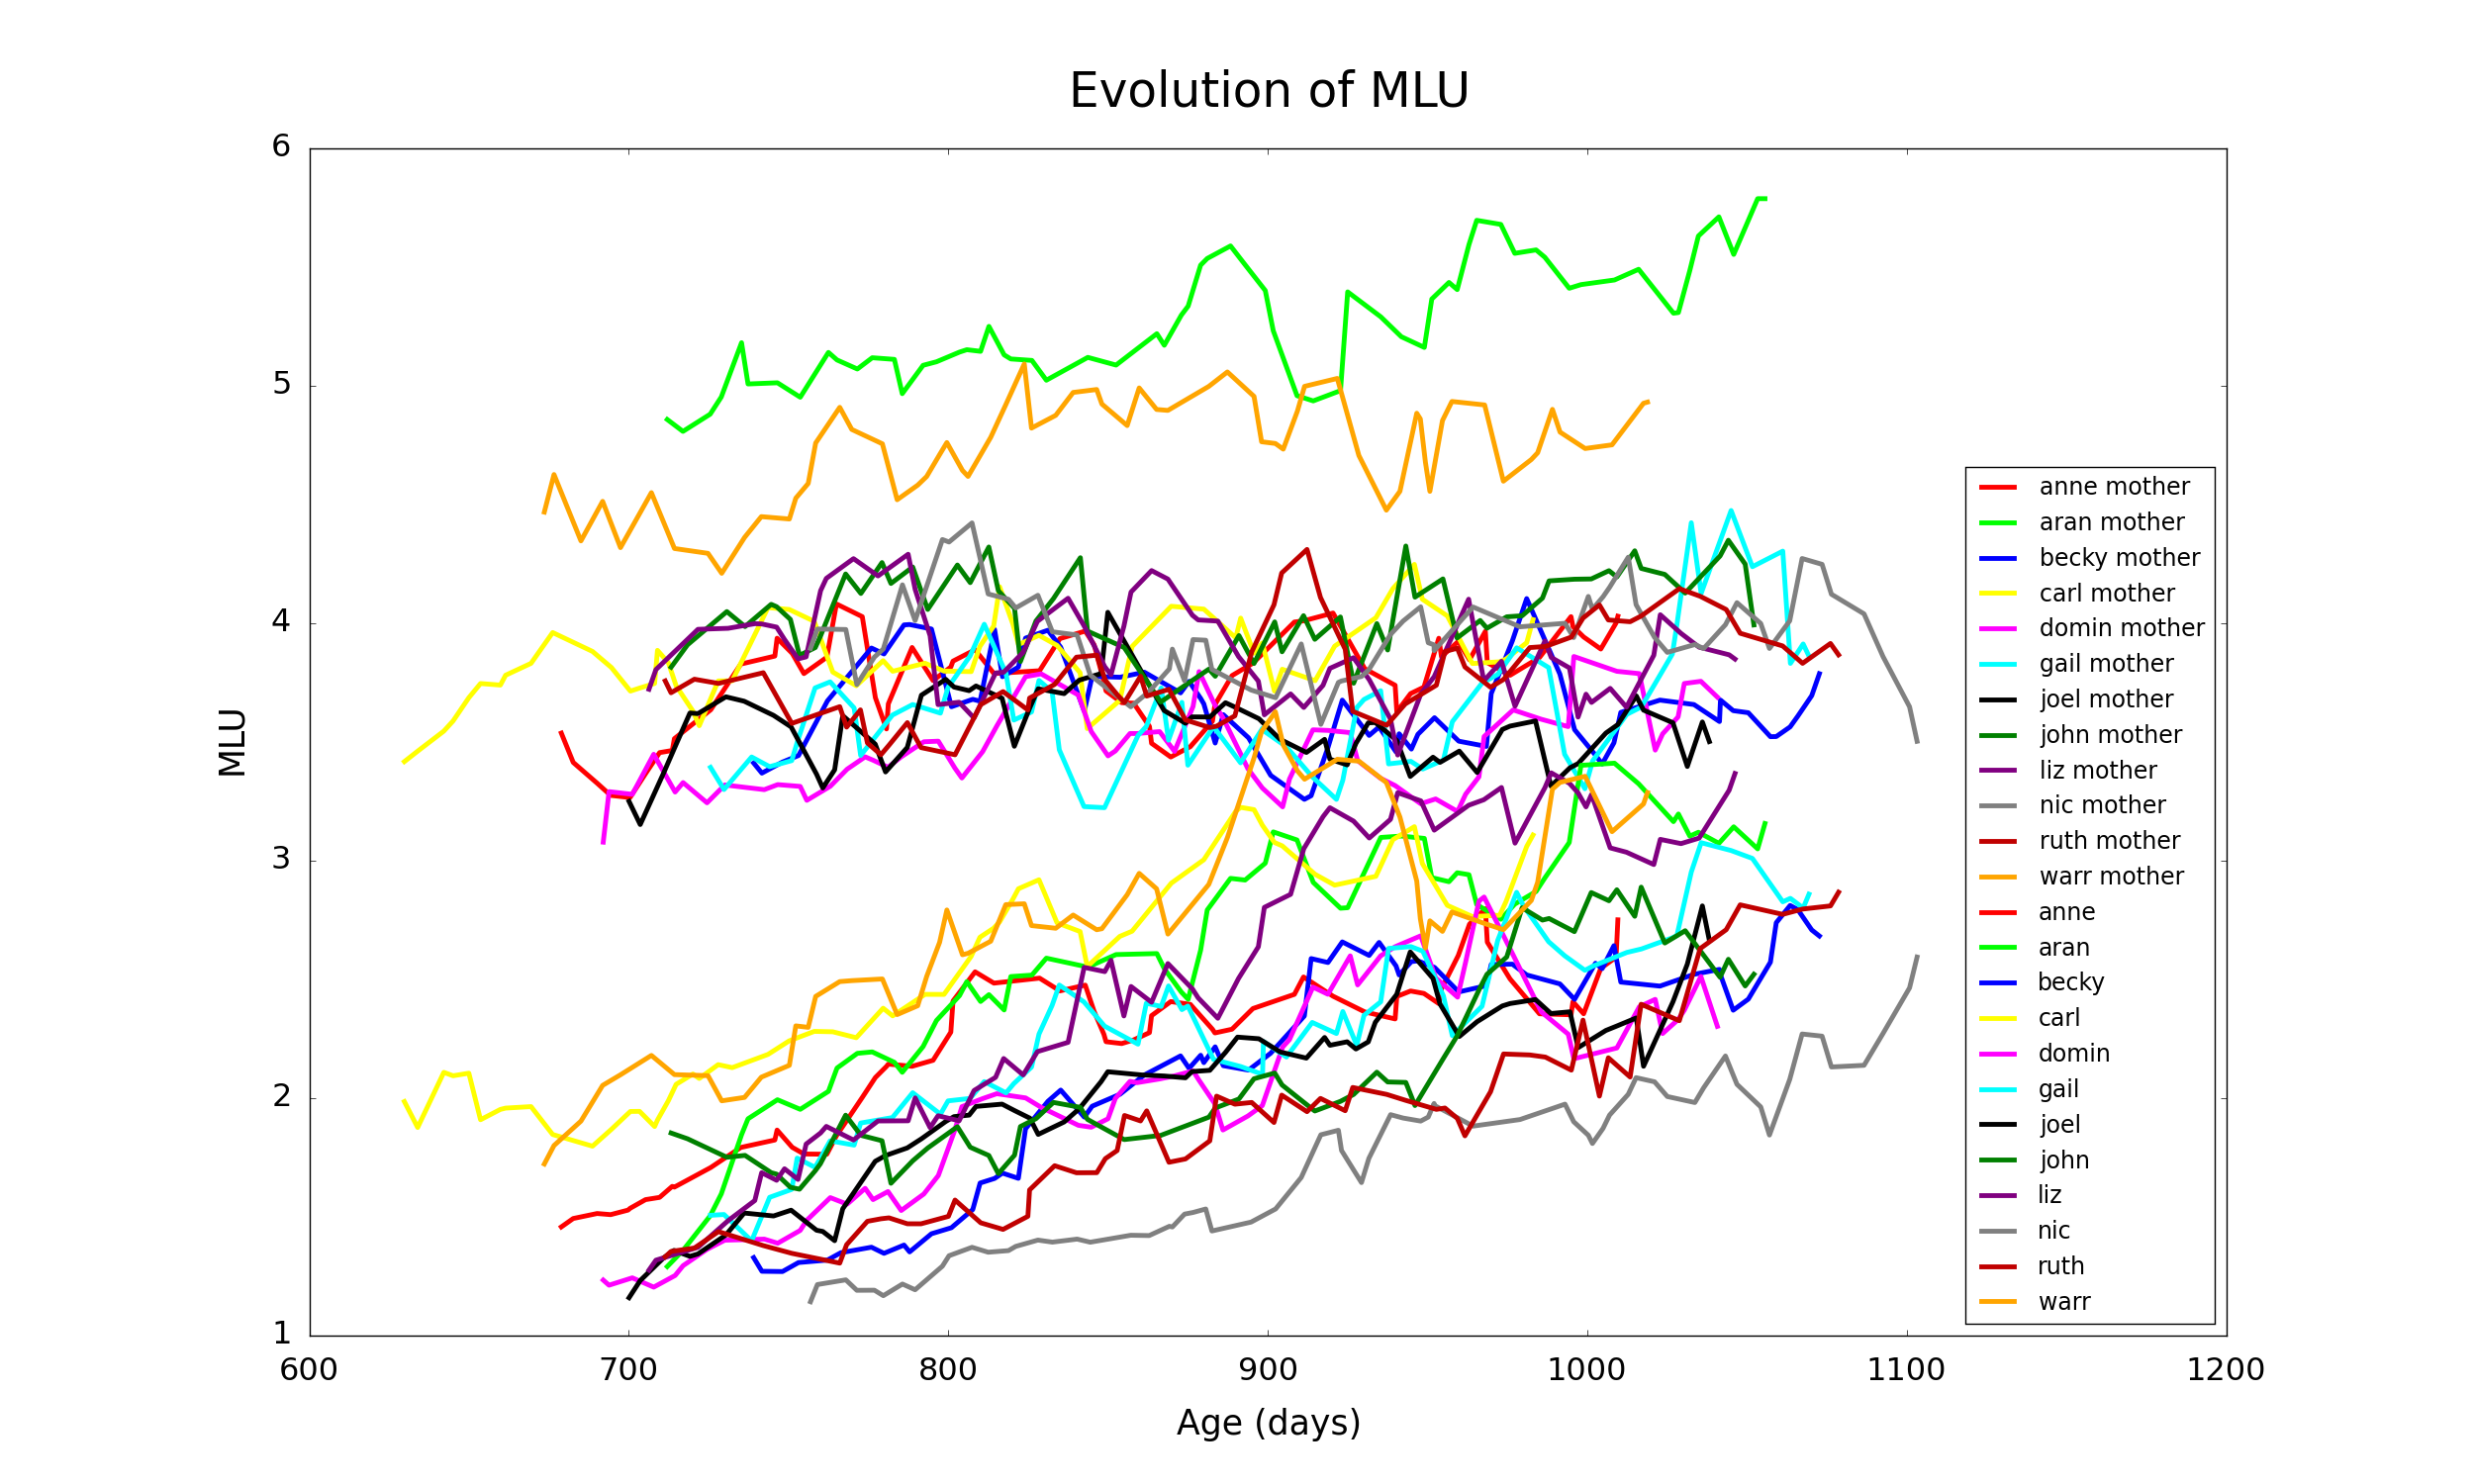
\includegraphics[width=.325\textwidth]{syntactic_evolution.png}
\end{tabular}
\caption{Evolution of the measures under consideration as a function of the children's ages, for the children (top row) and their mothers (bottom row). The total number of words produced are plotted in the left column, the lexical diversities in the middle column, and the MLUs in the right column.}
\label{fig:evolution}
\end{figure}
\end{block}

\begin{block}{Results}
\begin{figure}
\begin{tabular}{ccc}
{\bf (a)} & {\bf (b)} & {\bf (c)} \\
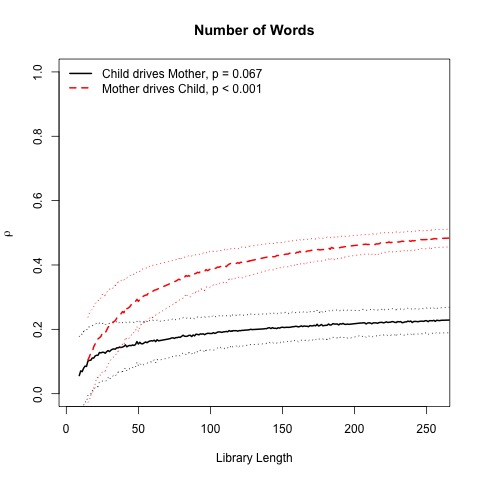
\includegraphics[width=.32\textwidth]{N_Words_Cause.jpg} &
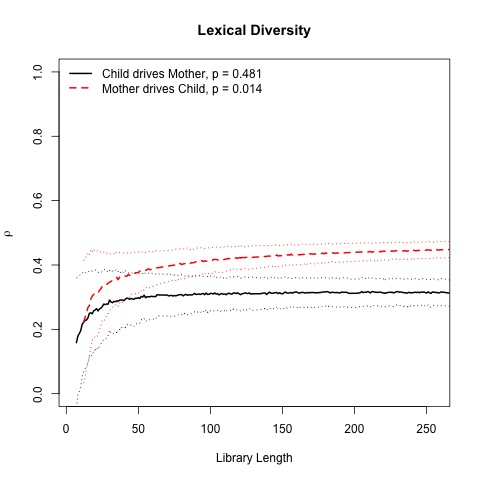
\includegraphics[width=.32\textwidth]{Lexical_Cause.jpg} &
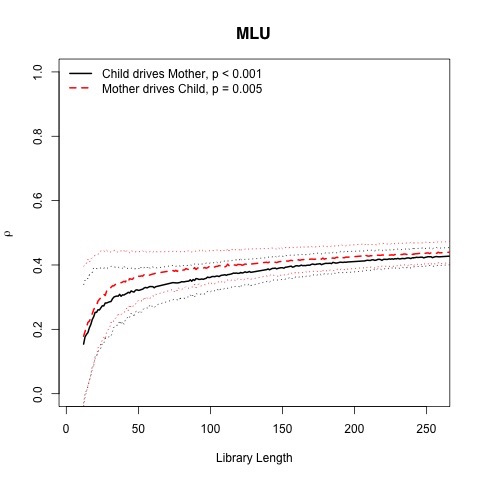
\includegraphics[width=.32\textwidth]{Syntactic_Cause.jpg}
\end{tabular}
\caption{For each of the measures considered, the panels plot the evolution of Pearson’s correlation coefficient ($\rho$) between the predicted and predicting shadow manifolds. The dashed lines denotes the standard deviation of the estimates. The $p$-values indicated in the legend were obtained by the bootstrapping procedure described by Clark et al. (2015). A value of $\rho$ significantly increasing with library length is mCCM’s indication of causality between two variables.}
\label{fig:results}
\end{figure}
\end{block}

\begin{block}{References}

\end{block}

\end{textblock}

\end{frame}
\end{document}
